%% generato automaticamente da tools/build_tex.py --- non modificare
\chapter{La gaussiana dal cerchio}
\label{cap:gauss}
\quaderno{gauss.dfw}{15 Sep 2010}{14}

Settembre 2010. Quattordici espressioni con un obiettivo dichiarato dal nome del file e mai scritto per esteso: arrivare alla funzione degli errori partendo dalla parametrizzazione razionale del cerchio. Il collegamento fra le due cose esiste ed è semplice — la gaussiana è la formula del cerchio letta sull'asse immaginario — ma il tratto finale, quello che porterebbe a $\operatorname{erf}$, resta aperto.

\section{La parametrizzazione razionale}

La prima riga contiene quattro scritture della stessa cosa, ed è il punto di partenza. Posto $s=\tan(t/2)$, si ha $\mathrm{e}^{\mathrm{i}t}=\dfrac{(1+\mathrm{i}s)^2}{1+s^2}$: è la sostituzione di Weierstrass, quella che rende razionale ogni integrale trigonometrico.

\begin{espr}{1}{User}{}
\begin{align*}
& \mathrm{e}^{\mathrm{i}\, t} \\
=\;& \frac{\left(1 + \mathrm{i}\, \tan\!\left(\frac{t}{2}\right)\right)^{2}}{1 + \tan^{2}\!\left(\frac{t}{2}\right)} \\
=\;& \frac{\left(1 + \mathrm{i}\, \tan\!\left(\frac{t}{2}\right)\right)^{2}}{\left|1 + \mathrm{i}\, \tan\!\left(\frac{t}{2}\right)\right|^{2}} \\
=\;& \operatorname{sgn}^{2}\!\left(1 + \mathrm{i}\, \tan\!\left(\frac{t}{2}\right)\right) \\
=\;& \frac{\cos\!\left(t\right) + 1}{2}\, \left(1 + \mathrm{i}\, \tan\!\left(\frac{t}{2}\right)\right)^{2}
\end{align*}
\end{espr}
Quattro scritture equivalenti dell'esponenziale immaginario, tutte fondate sulla tangente dell'angolo metà.

\begin{espr}{2}{User}{\verificata}
\[
1 + \tan^{2}\!\left(\frac{t}{2}\right) = \frac{2}{\cos\!\left(t\right) + 1}
\]
\end{espr}
L'identità che lega la secante quadra dell'angolo metà al coseno dell'angolo intero.

\begin{espr}{3}{User}{}
\[
\int 1 + \tan^{2}\!\left(\frac{t}{2}\right) \,\mathrm{d}t = 2\, \tan\!\left(\frac{t}{2}\right)
\]
\end{espr}
La stessa quantità è la derivata di $2\tan(t/2)$: l'osservazione serve alla riga seguente.

\begin{espr}{4}{User}{\verificata}
\begin{align*}
& \mathrm{e}^{\mathrm{i}\, t} \\
=\;& \frac{\left(1 + \mathrm{i}\, \tan\!\left(\frac{t}{2}\right)\right)^{2}}{\frac{\mathrm{d}}{\mathrm{d}t}\!\left[2\, \tan\!\left(\frac{t}{2}\right)\right]}
\end{align*}
\end{espr}
L'esponenziale scritto come rapporto fra un quadrato e una derivata.


La verifica è diretta: $(1+\mathrm{i}s)^2=1-s^2+2\mathrm{i}s$, e dividendo per $1+s^2$ si ottengono esattamente $\cos t$ e $\sin t$ in funzione della tangente dell'angolo metà. La riga $\#2$ registra l'identità $1+\tan^2(t/2)=2/(1+\cos t)$ e la riga $\#3$ osserva che quella stessa quantità è la derivata di $2\tan(t/2)$. La riga $\#4$ ne trae la scrittura più suggestiva: l'esponenziale immaginario è un quadrato diviso per una derivata.

\section{Il passaggio all'argomento immaginario}

Una riga sola, ed è il centro del quaderno.

\begin{espr}{5}{Sub(User)}{\verificata}
\begin{align*}
& \mathrm{e}^{\mathrm{i}\, \left(\mathrm{i}\, x^{2}\right)} \\
=\;& \frac{\left(1 + \mathrm{i}\, \tan\!\left(\frac{\mathrm{i}\, x^{2}}{2}\right)\right)^{2}}{1 + \tan^{2}\!\left(\frac{\mathrm{i}\, x^{2}}{2}\right)} \\
=\;& \frac{\cos\!\left(\mathrm{i}\, x^{2}\right) + 1}{2}\, \left(1 + \mathrm{i}\, \tan\!\left(\frac{\mathrm{i}\, x^{2}}{2}\right)\right)^{2}
\end{align*}
\end{espr}
La riga centrale: con $t=\mathrm{i}x^2$ il primo membro è la gaussiana, e il secondo si riduce a $\left(\cosh-\sinh\right)^2$.


Sostituendo $t=\mathrm{i}x^2$ il primo membro diventa $\mathrm{e}^{\mathrm{i}\cdot\mathrm{i}x^2}=\mathrm{e}^{-x^2}$: la gaussiana. E il secondo membro si semplifica altrettanto bene. Poiché $\tan(\mathrm{i}u)=\mathrm{i}\tanh u$, si ha $1+\mathrm{i}\tan\!\left(\mathrm{i}\tfrac{x^2}{2}\right)=1-\tanh\tfrac{x^2}{2}$ e $1+\tan^2\!\left(\mathrm{i}\tfrac{x^2}{2}\right)=\operatorname{sech}^2\tfrac{x^2}{2}$, per cui il rapporto vale
\[
  \left(1-\tanh\tfrac{x^2}{2}\right)^2\cosh^2\tfrac{x^2}{2}
  =\left(\cosh\tfrac{x^2}{2}-\sinh\tfrac{x^2}{2}\right)^2
  =\mathrm{e}^{-x^2}.
\]
La gaussiana è dunque, letteralmente, la stessa formula che parametrizza il cerchio, letta lungo l'asse immaginario. È il risultato per cui il quaderno esiste.

\section{L'integrale della funzione segno}

Il tentativo di chiudere il cerchio parte da un'osservazione elementare e passa per un integrale che Derive risolve in una forma inaspettata.

\begin{espr}{6}{User}{}
\[
\int \operatorname{sgn}\!\left(x\right) \,\mathrm{d}x = \left|x\right|
\]
\end{espr}
Il modello da imitare: la primitiva del segno è il valore assoluto.

\begin{espr}{7}{User}{}
\[
\operatorname{sgn}\!\left(1 + \mathrm{i}\, \tan\!\left(\frac{t}{2}\right)\right)
\]
\end{espr}
La funzione segno del numero che parametrizza il cerchio: ha modulo uno ma è discontinua.

\begin{espr}{8}{Int(\#7,t)}{}
\[
\int \operatorname{sgn}\!\left(1 + \mathrm{i}\, \tan\!\left(\frac{t}{2}\right)\right) \,\mathrm{d}t
\]
\end{espr}
Se ne chiede la primitiva.

\begin{espr}{9}{Simp(Int(\#7,t))}{}
\[
-4\, \left\lfloor \frac{1}{2} - \frac{t}{2\, \pi} \right\rfloor + \frac{\sqrt{2}\, \sin\!\left(t\right)}{\sqrt{\cos\!\left(t\right) + 1}} - \sqrt{2}\, \mathrm{i}\, \sqrt{\cos\!\left(t\right) + 1}
\]
\end{espr}
La risposta. Il termine con la parte intera raccorda i tratti fra un salto e il successivo.

\begin{figure}[htbp]
  \centering
  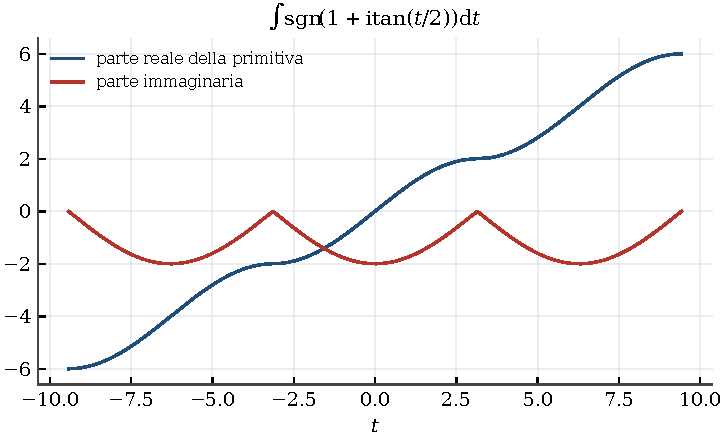
\includegraphics[width=0.86\linewidth]{../figures/gauss_sign.pdf}
  \caption{La primitiva della riga $\#9$. La parte reale sale a gradini raccordati — è l'effetto del termine con la parte intera — mentre la parte immaginaria è periodica e vale $-2\left|\cos(t/2)\right|$.}
  \label{fig:gauss_sign}
\end{figure}
\begin{espr}{10}{User}{}
\[
-4\, \left\lfloor \frac{1}{2} - \frac{t}{2\, \pi} \right\rfloor + \frac{\sqrt{2}\, \sin\!\left(t\right)}{\sqrt{\cos\!\left(t\right) + 1}}
\]
\end{espr}
La sola parte reale della primitiva.

\begin{espr}{11}{User}{}
\[
\operatorname{erf}\!\left(t\right)
\]
\end{espr}
La funzione degli errori, scritta da sola: è l'obiettivo verso cui il quaderno si sta muovendo.


La riga $\#6$ ricorda che la primitiva della funzione segno è il valore assoluto: è il modello di quello che si vorrebbe ottenere, una funzione non elementare come primitiva di una elementare a tratti.

La riga $\#9$ è la risposta di Derive all'integrale della riga $\#8$, e il termine con la parte intera merita una spiegazione. La quantità $\mathrm{sgn}\!\left(1+\mathrm{i}\tan\tfrac{t}{2}\right)$ ha modulo uno, e verrebbe da scrivere che vale $\mathrm{e}^{\mathrm{i}t/2}$ — ma non è così, perché il numero $1+\mathrm{i}\tan(t/2)$ ha sempre parte reale uguale a $1$ e quindi argomento confinato fra $-\pi/2$ e $\pi/2$. La funzione è discontinua, salta di $\pi$ ogni volta che la tangente diverge, e la primitiva deve rimettere insieme i tratti: è questo il compito del termine $-4\left\lfloor\tfrac12-\tfrac{t}{2\pi}\right\rfloor$, che aggiunge una costante diversa su ogni periodo. Le due parti restanti, riscritte con $\cos t+1=2\cos^2(t/2)$, valgono $2\sin\tfrac t2\,\mathrm{sgn}\!\left(\cos\tfrac t2\right)$ e $-2\mathrm{i}\left|\cos\tfrac t2\right|$.

\section{Il tratto che resta aperto}

Le ultime tre righe applicano al caso quadratico la stessa costruzione e si fermano lì.

\begin{espr}{12}{User}{}
\[
\int \operatorname{sgn}\!\left(1 + \mathrm{i}\, \tan\!\left(\frac{t^{2}}{2}\right)\right) \,\mathrm{d}t
\]
\end{espr}
La stessa costruzione con argomento quadratico.

\begin{espr}{13}{Simp(User)}{}
\[
\frac{\sqrt{2}\, \int \sqrt{\cos\!\left(t^{2}\right) + 1} \,\mathrm{d}t}{2} + \frac{\sqrt{2}\, \mathrm{i}\, \int \frac{\sin\!\left(t^{2}\right)}{\sqrt{\cos\!\left(t^{2}\right) + 1}} \,\mathrm{d}t}{2}
\]
\end{espr}
Che si spezza in due integrali di tipo Fresnel, nessuno dei quali elementare.

\begin{espr}{14}{User}{}
\[
\int \operatorname{sgn}\!\left(1 + \mathrm{i}\, \tan\!\left(\frac{\mathrm{i}\, t^{2}}{2}\right)\right) \,\mathrm{d}t
\]
\end{espr}
Il tentativo con argomento immaginario, lasciato senza risposta. Qui la funzione segno vale identicamente uno e la costruzione si svuota.


Sostituendo $t\to t^2$, l'integrale si spezza nelle due parti della riga $\#13$, che sono integrali di tipo Fresnel: la stessa famiglia incontrata tre mesi prima in \dfw{cost\\textasciicircum{}{}2.dfw} (capitolo~\ref{cap:cost2}). La riga $\#14$ tenta il passaggio all'argomento immaginario, quello che secondo la riga $\#5$ dovrebbe produrre la gaussiana e quindi, integrando, la funzione degli errori. Derive non porta a termine il calcolo e il quaderno si interrompe.

Vale la pena notare che il passaggio non è solo un problema di software. Con argomento immaginario la quantità $1+\mathrm{i}\tan\!\left(\mathrm{i}t^2/2\right)=1-\tanh(t^2/2)$ è reale e positiva, quindi la sua funzione segno vale identicamente uno e l'integrale è banalmente $t$: la costruzione perde per strada proprio l'informazione che serviva. Per ottenere $\operatorname{erf}$ occorre integrare la gaussiana, non il segno di ciò che la genera.

\section*{In sintesi}
\addcontentsline{toc}{section}{In sintesi}

Il risultato del quaderno è che la gaussiana è la parametrizzazione razionale del cerchio valutata lungo l'asse immaginario: $\mathrm{e}^{-x^2}=\left(1-\tanh\tfrac{x^2}{2}\right)/\left(1+\tanh\tfrac{x^2}{2}\right)$. Preso da solo è un'osservazione semplice; è però un pezzo di un'idea che attraversa cinque quaderni, l'esponenziale scritto con la tangente del semiangolo, che la nota a corredo di questa edizione ricostruisce per intero. Il programma che l'autore si era dato — arrivare da lì alla funzione degli errori — non viene completato, e la ragione non è la debolezza del calcolatore ma la struttura del problema: la funzione segno, che nel caso circolare portava l'informazione utile, nel caso immaginario diventa costante.

